\documentclass[sigconf]{acmart}

\usepackage{hyperref}

\usepackage{endfloat}
\renewcommand{\efloatseparator}{\mbox{}} % no new page between figures

\usepackage{booktabs} % For formal tables

\settopmatter{printacmref=false} % Removes citation information below abstract
\renewcommand\footnotetextcopyrightpermission[1]{} % removes footnote with conference information in first column
\pagestyle{plain} % removes running headers

\begin{document}
\title{Big Data Applications in Fraud Detection in Insurance}

\author{Mrunal L Chaudhary}
\affiliation{%
  \institution{Indiana University}
  \city{Bloomington} 
  \state{Indiana} 
}
\email{mchaudh@iu.edu}

% The default list of authors is too long for headers}
\renewcommand{\shortauthors}{B. Trovato et al.}


\begin{abstract}
Insurance companies today are incurring a loss in billions of dollars every year because of frauds happening in filing claims, paying premiums, filling applications etc. Detecting frauds manually or by other traditional means is an impossible task since magnanimous amounts of data is getting generated every day and fraudsters change their strategies very quickly. For handling such a humongous amount of data, performing real time analysis on it, and getting accurate outputs; it is imperative that a robust, flexible and scalable technology be used which can detect frauds on the fly. Big data provides just the platform needed to perform analysis of such high complexity.
\end{abstract}

\keywords{i523, HID205, Insurance, Fraud detection in insurance, Predictive analysis}


\maketitle

\section{Introduction}
The fact that technology is evolving at the fastest pace in the history of mankind needs no more of a proof than a mere glance of eyes around our surroundings. But like everything else, it is a double-edged knife and this advancement in technology comes at a cost of benefiting the fraudsters of the society. A fraud can be defined as a "wrongful or criminal deception intended to result in financial or personal gain". And while they are rampant in almost every field, there is no surprise that the field of insurance too has been affected by them. Traditionally, Insurance industry estimated that frauds account for about 10 percent of the total losses incurred by them which is equivalent to billions of dollars, and these numbers are only rising.\cite{link1} As these fraudsters are getting smarter, and well equipped with technology, insurance companies are facing difficulties in preventing and detecting the fraudulent activities with the traditional ways. Though the proliferation of modern technology aids the fraudsters in generating sophisticated fraud techniques, the advancement in technology has enabled better and smarter approaches in detecting fraud. In a world where data is getting generated at a break-neck speed, transactions are digitally documented in one way or the other, evidence is just hidden in the data for aiding the investigators to damage the fraudulent activities. The question then that needs to be addressed is- "how to easily and quickly find that evidence?"\cite{link4}

\section{Background}
Most of the insurance frauds are committed in the fields of Health care, auto insurance and workers' compensation. These frauds can either be 'hard' or 'soft'. Hard frauds occur when someone on purpose makes up claims or fakes an accident. Soft fraud occurs when they inflate the amount of a legitimate claim. The people who do insurance frauds can either be organized criminals who draw large sums of money from fraudulent claims, professionals who add on to legitimate claims or ordinary people who just want to cover the amount of premiums or deductibles. The parties that are most affected by frauds are consumers who have to pay higher insurance premiums for compensating the losses from frauds, and medical professionals who are concerned of tarnishing their reputation.\cite{link6}


\section{Reasons for failure of traditional approaches}
The natural question then that comes to the mind is, "Why are the traditional approaches to detect fraud inadequate?" The rate at which this voluminous data is getting generated is just impossible to efficiently and accurately process manually. The data sources that get generated were far too large and were changing far too often so as to be helpful in scoring the fraud the traditional way, since they used batch processing which took hours or even days together to run. Moreover, the insurance firms used red-flag business rules for suspicious claim detection. Thus, using sampling techniques was bound to skip some frauds and introduce errors. Also, the data generated by insurance companies is ever evolving and changing, and the traditional approaches are not sustainable to process data at real time. Thus tweaking of parameters in the fraud detection algorithm was an impossible task since it requires a lot of processing time. Hence, traditional approaches to fraud detection lacked both- the flexibility and the scalability.\cite{link3} And lastly, traditional approaches only looked at the structured data since the fraud detection systems were not equipped to handle unstructured data, thereby eliminating a huge subset of data, and making the critical decisions on incomplete information.\cite{link5}

\section{Challenges faced in Fraud detection}
It is widely recognized that the volume of data is increasing at breakneck speed. In fact experts believe that the amount of data that has been amassed in the last two years- a zettabyte- is more than the data that has been generated since the dawn of the human civilization.\cite{link2} But more astonishing than this is that the volume is only one part of the entire equation. With volume, big data deals with velocity and variety. Insurers can access a variety of information that is ever increasing and can be accessed through machine-to-machine data, social media and customer feedback and reports in the form of unstructured data. Also photos and videos are another rich source of visual media information that the insurers can lay their hands over. And this information is ever changing and increasing. Thus, dealing with the velocity and variety of the voluminous data are challenges in themselves. \cite{link3}

\section{Advantages of using big data in fraud detection}
One of the biggest advantage that high-performance analytics allows is the ability to use the ever-changing and increasing data sources previously ignored because of the lack of sophisticated tools for handling big data. With the advent of high-performance analytics, billions of rows of data can be processed in a matter of seconds. Thus, insurers can determine fraud scoring in real time. Insurers can now test certain approaches in real time and constantly tweak the parameters for maximizing the output of the fraud detection algorithms. Since high performance analytics can process a magnanimous amount of data in mere seconds, sampling of data is no more needed. Hence the error introduced by sampling can be completely avoided by using big data technologies. With the help of high performance analytics, sophisticated models like supervised predictive modeling, data mining, social network analysis, social customer relationship management, etc. can be implemented to improve the process of analysis. With the arrival of big data, the process of fraud detection can be completely revolutionized. 
"High-performance analytics is not just another technology fad. It represents a revolutionary change in the way organizations harness data. With new distributed computing options like in-memory processing on commodity hardware, insurers can have access to a flexible and scalable real-time big data analytics solution at a reasonable cost. This is sure to change the way insurance companies manage big data across their business- especially in detecting fraud."\cite{link3}

\section{Role of Analytics in Fraud Detection} 
Traditionally, insurance companies have used Statistical models for the identification of frauds in claiming insurance policies. There are several challenges that these models pose. First, since Sampling of data is used to analyze data, possibility of one or two frauds not getting detected is very high. Second this method relies on already existing data in fraud cases, hence every time a new fraud is committed the insurance company has to bear the costs for the first time. And most importantly the traditional methods work in silos, and hence are not scalable to handle the rapidly growing information from different sources. Analytics therefore play an important role in fraud detection by addressing these issues. The key benefits are\\
1.Analytics help in the detection of low key incidence events \\
2.Analytics helps in effective integration of data. Third party data may have important predictive value such as criminal records, bankruptcies, liens, bill review data, etc which can help in determining behaviors prevalent in fraudsters.\\
3.Since most of the data related to fraudsters like third party reports, is available in unstructured format, which is not saved in most of the data warehouses, text analysis can play an important role in providing valuable insights in fraud detection\cite{link7}

\section{INNOVATIVE FRAUD DETECTION METHODS}
\subsection{SNA(Social Network Analysis)}
"SNA allows the company to look through large amounts of data to show relationships via links and nodes. The SNA tool combines a hybrid approach of analytical methods. This approach includes business rules, statistical methods, pattern analysis, and network linkage analysis to uncover large amounts of data to show relationships via links". 
SNA works like this: After feeding the data into an ETL(extract, transform and load) tool, the Analytics team scores the risk of fraud by prioritizing the likelihood based on the history of the claimant, relationship with other fraudsters, multiple claims, etc. The Fraud Identification and Predictive Modeling process is an integrated framework of technologies like sentiment analysis, text mining, content categorization, social network analysis. Thus, by doing this, the insurer can rate each claim. A fraudulent claim can therefore be indicated by a high rating. The correctly identified frauds are then added into the business use case system.\cite{link7}
\begin{figure}
  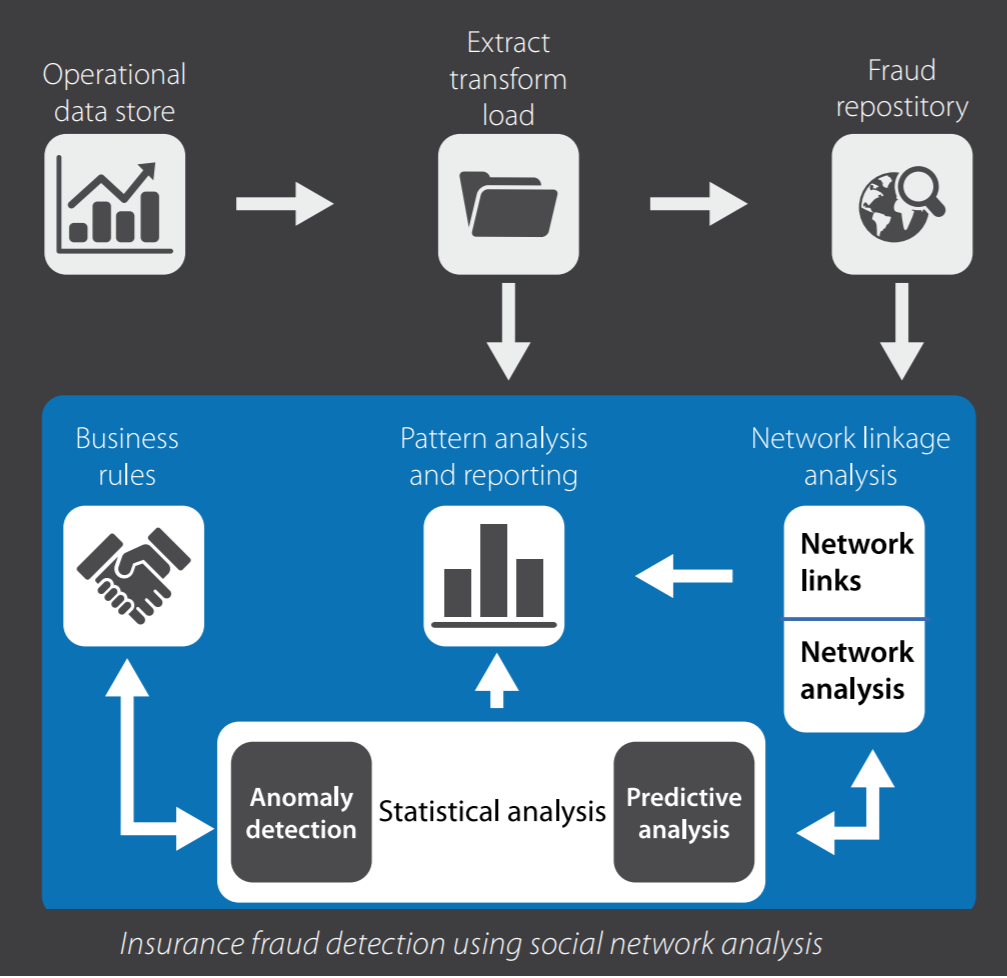
\includegraphics[width=\linewidth]{images/SNA_image1.png}
  \caption{Social Network Analysis Flow chart}
  \label{fig:Social Network Analysis flowchart}
\end{figure}
\subsection{Predictive Analysis for Big Data}
Predictive analysis makes use of text and sentiment analysis to go through big data for fraud detection. Big data helps in proactively detecting the fraudulent cases by quickly sifting through the large claim reports which are unstructured in nature. An important point to note is that people committing frauds mostly alter their story with time. And these clues are hidden in the log reports submitted by the claim adjusters. The computing system based on the business rules can spot the evidence of the fraudulent claims easily with the help of text and sentiment analysis. \cite{link7}
\begin{figure}
  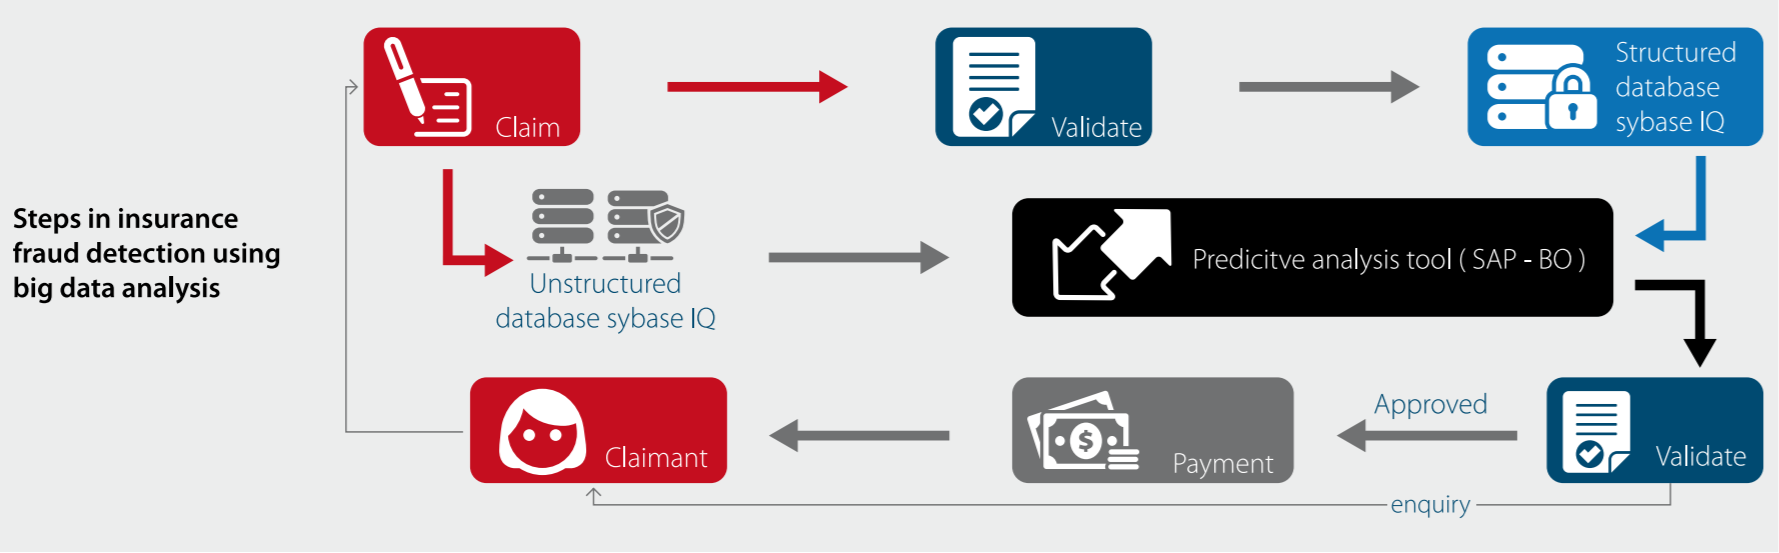
\includegraphics[width=\linewidth]{images/predictive_image1.png}
  \caption{Predictive Analysis Flow chart}
  \label{fig:Predictive Analysis flowchart}
\end{figure}
\subsection{Social Customer Relationship Management}
The SCRM is a process that Companies should follow to link their CRM with social media to enable greater levels of transparency with their customers. This transparency is mutual in nature since it means insurance companies can trust their customers and vice-versa. The reference data which the company extracts from social media chatter using a 'listening tool', along with information stored in the company's existing CRM is fed into a case management system. This system then sends a response about whether the claim is fraudulent or not, which is confirmed by the investigators. \cite{link7}
\begin{figure}
  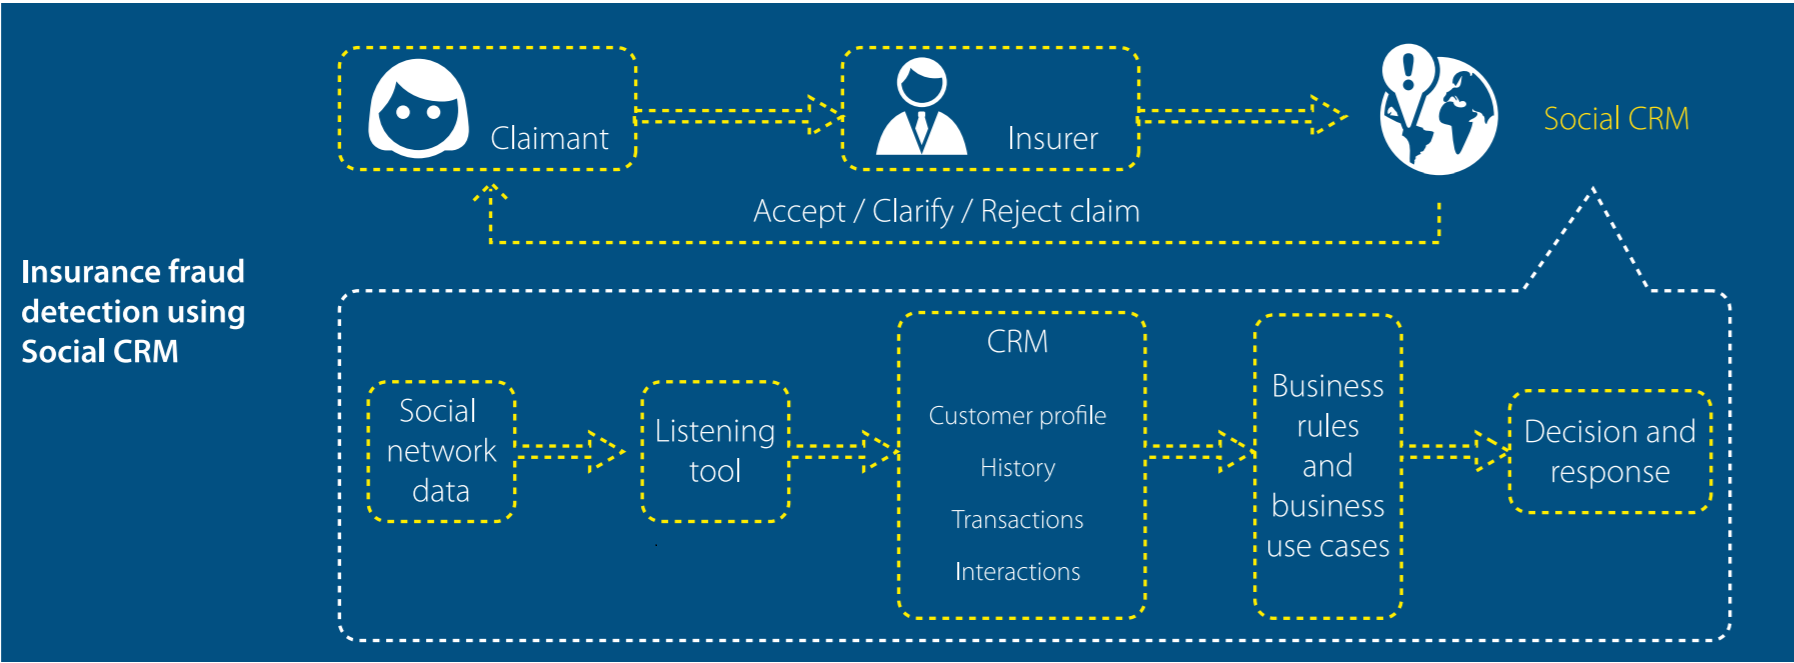
\includegraphics[width=\linewidth]{images/SCRM_image1.png}
  \caption{Social Customer Relationship Management Flow chart}
  \label{fig:Social Customer Relationship Management Flow chart}
\end{figure}
\\
\\
Most of the Insurance Fraud detection tools build a framework around the claim management vertical, but for building a more robust system, a holistic framework is needed, one which can identify potential areas for frauds like in application, premium, claims, etc. Following are the 10 steps for implementing the analytics of fraud detection.

\section{10-Step Implementation of Analytics in fraud detection}
\subsection{Perform SWOT}
Since there is an increasing awareness about the need for fraud detection systems amongst the insurance companies, before going for a solution, the company should perform a SWOT analysis of the existing fraud detection solutions and choose the one most aligned with its requirements.
\subsection{Build a dedicated Fraud Detection Team}
In a traditional set up, no team in an insurance company was held accountable for fraud detection. It is important to form a dedicated team for fraud detection which can be held responsible for frauds going unnoticed.
\subsection{Whether to build or buy	}
Once the first two steps are accomplished, an Insurance company needs to address the important question as to whether to buy a framework or to implement the analysis themselves. In case they decide to go for the latter, they need to be sure that they have the required skill set for building an in-house analytics solution. And if not, the insurance company should find an analytics solution that best fits the requirements of the company. 
\subsection{Clean data}
In this step, databases are integrated and redundancies are removed from data 
\subsection{Come up with relevant business rules}
Certain types of frauds are very industry or company specific. The insurance companies should use to their advantage the existing in-house domain expertise to define the business rules in order to build a robust fraud detection framework.
\subsection{Define Anomaly Detection thresholds}
The insurance companies need to carefully set the threshold for Anomaly detection. If set to a high value there is a chance that many fraudulent claims might go unnoticed and if set to a very low value, there is a definitive risk associated with wasting time. The threshold values should be decided after taking into consideration a number of factors like the type of insurance, the rate of fraudulent claims associated with it, the time available at disposal, etc
\subsection{Use Predictive Modelling}
The data mining tools should be utilized for building models that can produce scores for fraud propensity in regard with unidentified metrics. The result thus can then be given for further analysis.
\subsection{Use Social Network Analysis}
SNA models relationships between various entities involved in claims and therefore, has proved to be very helpful in identifying the fraudulent activities. These entities can be anything from geographic location, car in case of car accidents, age groups, financial status, phone numbers, etc. Through SNA it can be found out that the linkage between some entities is higher than the average connection numbers, thus indicating fraudulent activities
\subsection{Building a Social Customer Relationship Model}
The integrated case management systems allows the insurance companies to capture relevant findings to claims data, adjuster nodes, social media(both structured and unstructured), and network diagrams. Metrics, the key indicators of fraud can be easily tabulated for comparisons between entities or network at an individual level. The case management process ensures efficiency, full assessment of the investigative workload and the ROI.
\subsection{Forward looking Analytic solutions}
For building a truly robust system the insurance companies should keep looking for additional third-party sources of data and their integration with existing solutions for increasing the efficiency of the fraud detection system. Also, they should always keep in mind the issue of scalability. With the ever-increasing data, the system should be such that it can handle the size of the data.
The above system can robustly analyze the unstructured data presented in the claims report of the claim adjuster, the claims given by the claimants and other third-party reports. It can shortlist the at risk customers by performing sentiment analysis on the claims report. It can identify complex patterns of fraudulent claims and warn about the potential issues of fraudulent claims. \cite{link7}

\section{Concerns related to Fraud Detection Systems}
Though Fraud detection system have become pretty robust and sophisticated, there are still come issues that need to be addressed which are the following:
\begin{itemize}
  \item The data that is collected by the insurers can be properly utilized. But the issue of authenticity of the data needs to be addressed
  \item Most of the modelling techniques are highly dependent on the past behaviors of the fraudsters. But their behavior changes so quickly that it makes the whole analysis worthless. Evaluating the quality of the data therefore is a huge struggle
  \item No matter how advanced the fraud detection tools becomes, there will always be a dependency on humans for converting the reports into actionable intelligence
  \item The loses incurred by the insurance firms are somewhat compensated by charging a higher amount for premiums, thus the insurance firms may lose out on loyal customers
  \item For fraud detection in claims, insurance firms may set up stricter review process which might lead to the loss of loyal customers since they may consider the review process a wastage of their time\cite{link8}
\end{itemize} 


\section{Conclusions}
The upsurge of analytics presents a world of almost limitless potential for insurance companies which have long held a foundation of information.  With the advent of big data, high-performance analytics technology represents an opportunity to completely revolutionize the way fraud is detected. Though Big Data applications in Insurance are still in the early stages, they have proved to be powerful to easily handle and process the velocity with which variety of voluminous data is getting generated. In the years to come, Big Data Analytics will find widespread applications in the field of insurance.


\bibliographystyle{ACM-Reference-Format}
\bibliography{report} 

\end{document}
